
\section{N-Body}
\label{sec:nbody}
In physics and astronomy, an N-body simulation is a simulation of a dynamical system of particles, usually under the influence of physical forces, such as gravity. N-body simulations are widely used tools in astrophysics, from investigating the dynamics of few-body systems like the solar system to understanding the evolution of the large-scale structure of the universe. They are also used to module fluids using smooth-particle hydrodynamics. 

\par 
This approach for discretisation is often referred to as a Lagrangian approach, where the observer follows an individual fluid parcel as it moves through space and time\footnote{Note that this in contrast to Eulerian specifications of the flow field, which we do not directly discuss in the assignment. In Eulerian codes, the fluid motion is evaluated at specific locations in the space, often evaluated using a mesh. This mesh can be regular or irregular, fixed or adaptive.}. The evolution of an individual particle's position gives the pathline of the parcel. 

\par 
An common use-case for an N-Body simulation is to follow the non-linear evolution of structure formation such as galaxy filaments and galaxy halos from the influence of dark matter on cosmological scales. An example of the output from the N-Body code provided in this assignment that mimics the distribution of matter in cosmological simulation is provided in Fig.~\ref{fig:nbody-distribution}.
\begin{figure}[!h]	
	\centering
	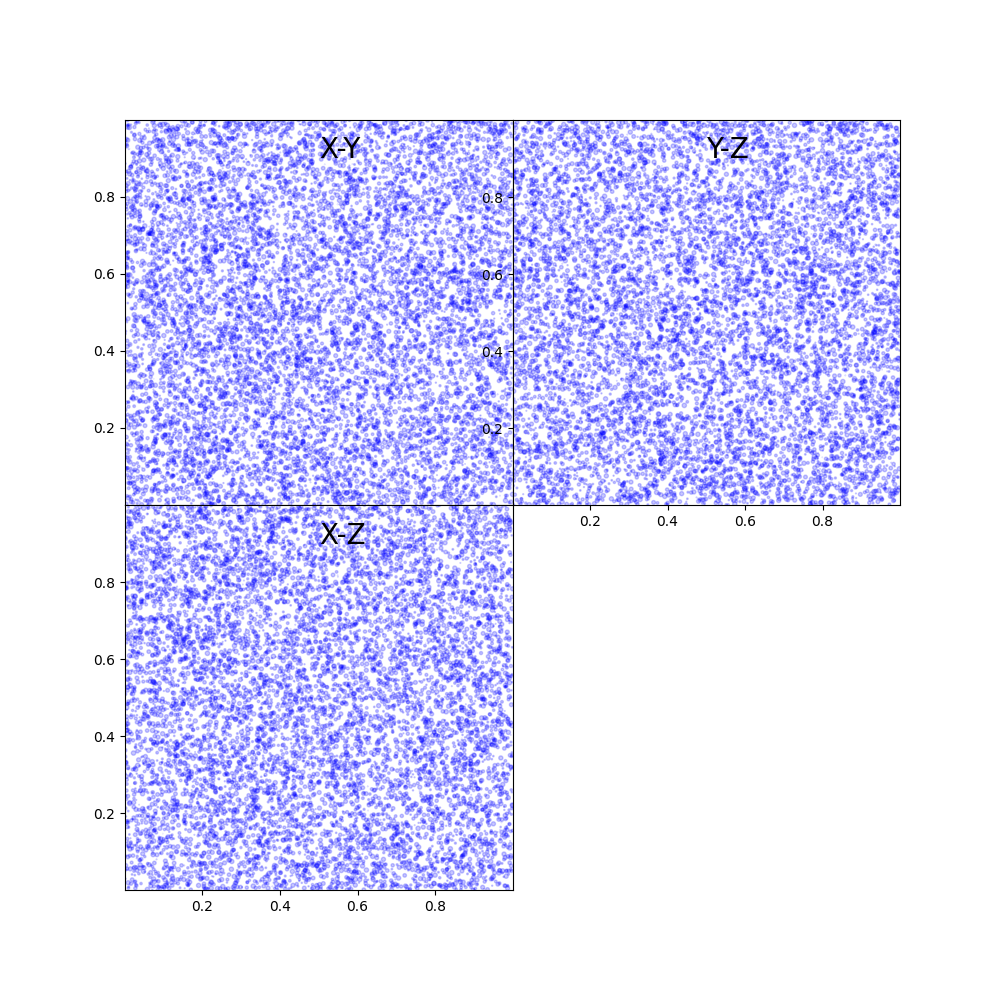
\includegraphics[width=0.4\textwidth, valign=c, clip=true, trim=2.cm 2.cm 2.cm 2.cm]{figs/nbody-scatter-plot.t-0.png}
	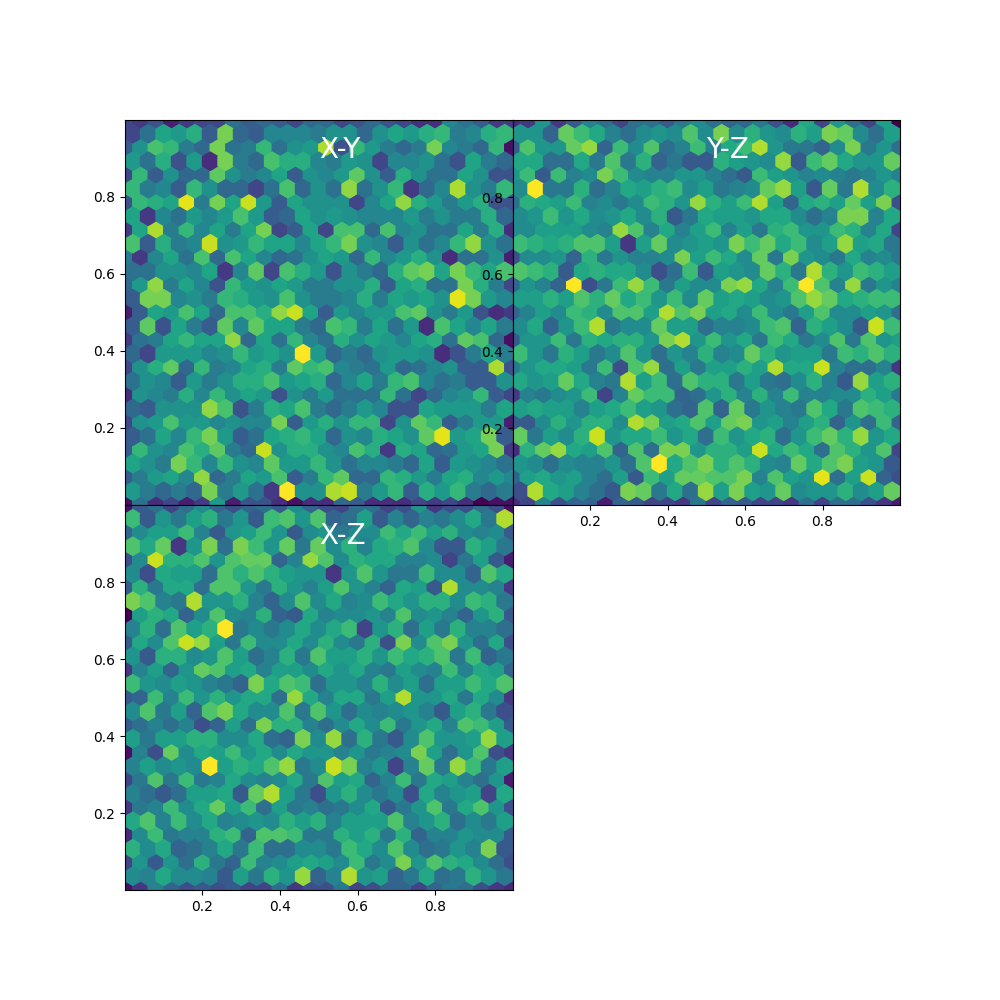
\includegraphics[width=0.4\textwidth, valign=c, clip=true, trim=2.cm 2.cm 2.cm 2.cm]{figs/nbody-density-plot.t-0.png}
	\caption{An example of a random particle distribution and the corresponding projected density field. We show $X-Y$, $X-Z$ and $Y-Z$ projections.}
	\label{fig:nbody-distribution}
\end{figure}

\par 
The basics of the computation for evolving particles at each individual time-step $\Delta t$ of the simulation are as follows:
\begin{itemize}
	\item {\color{ForestGreen}Acceleration} Calculate the acceleration, $\vec{a}_{\textrm{new}}$, on each individual particle. A simple N-body code can involve calculations that scale as $N^2$, where $N$ is the number of particles.
	\item {\color{CornflowerBlue}Velocity Update} Update the momentum of all the particles based on these forces, \\$\vec{p}_{\textrm{new}} = \vec{p}_{\textrm{old}} + \vec{a}_{\textrm{new}}\Delta t$
	\item {\color{Purple}Position Update} Update the positions of all the particles based on these momenta, \\$\vec{x}_{\textrm{new}} = \vec{x}_{\textrm{old}} + \vec{p}_{\textrm{new}}\Delta t$
\end{itemize}
There are issues with this simplified approach related to energy conservation primarily related to the time step. One can also use other techniques to reduce errors in the time-integration. 

\subsection{Impact of Time-steps}
\label{sec:nbody:timestep}
The time-integration technique is critical to conserving the total energy of the system and having the correct evolution. For example, the N-Body code provided in this assignment can evolve a system with a fixed time step or an adaptive time step. A poorly chosen fixed time step can result in the simulation not correctly evolving the system when the dynamical time is short, such as in close encounters of particles evolving under gravity as seen in Fig.~\ref{fig:nbody-orbits}. 
\begin{figure}[!h]	
	\centering
	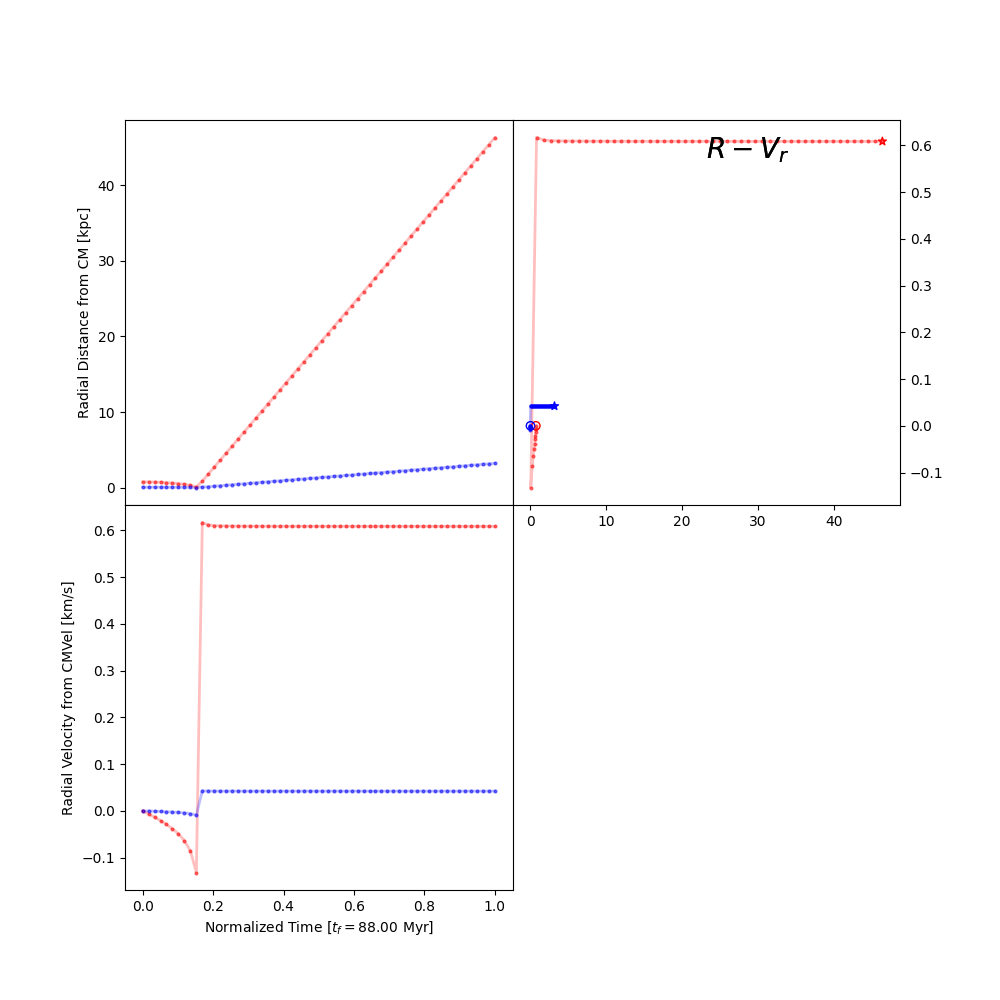
\includegraphics[width=0.4\textwidth, valign=c, clip=true, trim=1.cm 2.cm 1.cm 2.cm]{figs/nbody-phase-plot-rad-static.png}
	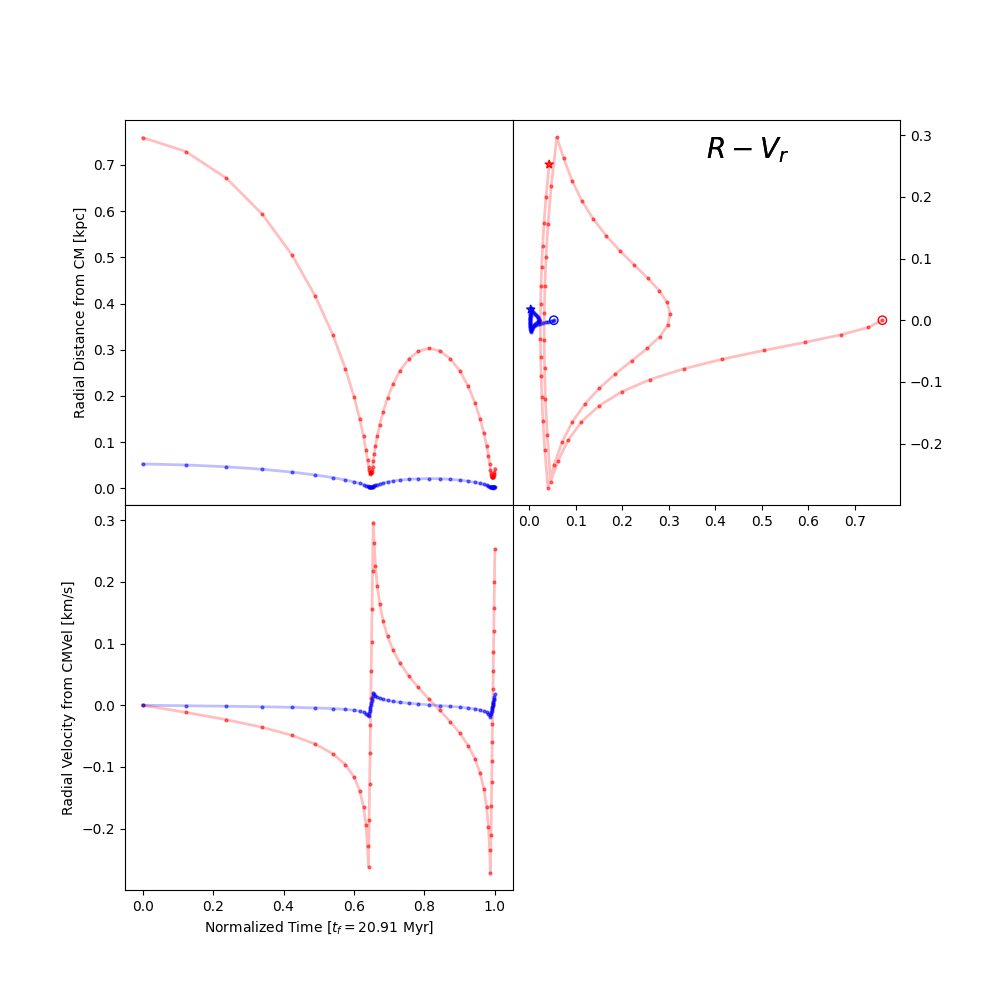
\includegraphics[width=0.4\textwidth, valign=c, clip=true, trim=1.cm 2.cm 1.cm 2.cm]{figs/nbody-phase-plot-rad-adaptive.png}
	\caption{Phase-space plots: We show an example of the impact time-steps can have on the evolution of the system comparing fixed time steps (left) to adaptive time steps (right). The left panels in each plot show the radial position and radial velocity as a function of time and the right panels show the radial velocity as a function of radial velocity, where the tracks start at a large circular marker and end at a $\star$.}
	\label{fig:nbody-orbits}
\end{figure}

\par 
Here we follow the radial position and velocity of two particles, one more massive (blue) than the other (red). The system is initialized such that the particles are in orbit around the common centre-of-mass. For the fixed time step, the simulation does not correctly follow the close encounter, moving the particle too much during this phase, resulting the lighter particle's having too much momentum after the encounter and streaming off unbound from the system as see in the left panel. 

\par 
An adaptive time step which is always set to some small fraction of the dynamical time of the system will correctly model the encounter. However, it is worth noting here that there are still issues with the energy of the system (see assignment questions). 

\subsection{Long-range forces}
\label{sec:nbody:longrange}
There are several challenges to modelling long-range forces. Long-range forces like the gravitational force are computationally expensive as the calculations scale as $\mathcal{O}(N^2)$, that is one must calculate the force between each pair of particles. Computational techniques can be used to reduce the scaling but require some approximations to be made (see assignment questions).

\par 
Correctly solving the force for periodic systems requires additional corrections as it is not computationally feasible to simple add more pairs where one has been shifted by the period. Such an approach would require terminating the number of additional particles out to some multiples of the period, introducing additional approximations. Instead, a typical approach is to break the force calculation into a shorter range and long (period) range set, often referred to as Ewald summation (see \href{https://en.wikipedia.org/wiki/Ewald_summation}{here}). 

\par 
Finally, there is added complexity to correctly calculating the true evolution of the system given the finite-speed of the force carrier. To accurately calculate long-distance forces a full general relativistic approach is required \cite{grnbody}. However, the difference between the accurate solution and an approximateive one where the force is transitted instantaneously can be small for forces that depend on radial distance of the form $r^{n}$, $n\leq-2$ since the long-range forces are small\cite{grcorrections}.

\subsection{Short-range forces}
\label{sec:nbody:shortrange}
Short range forces also face several challenges. The first is that the naive implementation would require 
$\mathcal{O}(N^2)$ radius calculation to see if a pair is within the short-range force before calculating said force. Computational techniques can be used to significantly reduce the computational cost of the local neighbour search, without requiring any approximations (see assignemnt questions).

\par 
These forces can also be subject to the speed of the force carrier and may also require corrections to accurately calculate the force. 

\section{Code Repository}\label{sec:code}
The code that forms the basis of the assignment contains the following 
\begin{itemize}
	\item basic files like a README, License
	\item \texttt{Makefile} setup to compile codes with a variety of different flags and features. For a quick tutorial on GNU Make, see \href{https://www.gnu.org/software/make/}{here}. Students are expected to be familiar with Make and the associated commands. Please familiarise yourself with this material. 
	\item source code in \texttt{src/*.f90} (\texttt{Fortran}). 
	\item documentation and \LaTeX\ source code in \texttt{docs}
	\item python scripts for visualisation. 
\end{itemize}
To familiarise yourself with the contents you can see what make options are available and browse the source directory. 
\begin{center}
\begin{minipage}{0.95\textwidth}
\small
\begin{minted}[frame=single,]{sh}
make allinfo # provides all the information of the commands listed below  
make configinfo # provides the different options available 
make makecommands # what you can make by typing these commands
make buildinfo # current compilers used
\end{minted}
\end{minipage}
\end{center}
You'll note that the make file is setup to accept command line arguments that can set compiler families such as \texttt{GCC}, \texttt{CRAY-GNU}, \texttt{CRAY} when you type \texttt{make configinfo}. Try the following
\begin{center}
\begin{minipage}{0.95\textwidth}
\small
\begin{minted}[frame=single,]{sh}
# use the GNU CC family of compilers, gcc, g++, & gfortran AND 
# compile the serial version of the code, both C and Fortran sources.
make COMPILERTYPE=GCC cpu_serial 
# use the GNU family of compilers with the Cray compiler wrappers 
# on Setonix and compile the openmp source codes (if present)
make COMPILERTYPE=CRAY-GNU cpu_openmp 
\end{minted}
\end{minipage}
\end{center}


\subsection{Source}
The common function calls with interfaces are listed in \texttt{src/common.f90} provides a module with the same set of interfaces and subroutines. 
\begin{center}
\begin{minipage}{0.95\textwidth}
\small
\begin{minted}[frame=single,]{fortran}
module nbody_common
    type Particle
        integer(8) :: ID
        real(8) :: mass
        real(8) :: radius
        real(8) :: position(3)
        real(8) :: velocity(3)
        real(8) :: accel(3)
        integer(8) :: PID
    end type Particle

    !   ascii mesh visualisation
    subroutine visualise_ascii_mesh(opt, step, parts)
    !   ascii visualisation (not implemented in full)
    subroutine visualise_ascii(opt, step, parts)
    ! no visualisation
    subroutine visualise_none(step)
    ! visualisation routine
    subroutine visualise(opt, step, parts)
    ! generate random IC
    subroutine generate_rand_IC(opt)
    ! generate random orbiting particles IC
    subroutine generate_orbit_IC(opt)
    ! generate IC
    subroutine generate_IC(opt, parts)
    ! UI
    subroutine getinput(opt)
    ! get some basic timing info
    real*8 function init_time()
    ! get the elapsed time relative to start
    subroutine get_elapsed_time(start)
end module
\end{minted}
\end{minipage}
\end{center}

\newpage
The main program consists of : 
\begin{center}
\begin{minipage}{0.95\textwidth}
\begin{minted}[frame=single,]{fortran}
    ! generate particles 
    call generate_IC(opt, parts)
    time1 = init_time()
    current_step = 0
    print *, "Running simulation for ", opt%nsteps
    ! run time integration for certain number of steps
    do while (current_step .ne. opt%nsteps)
            time2 = init_time()
            ! visualise if necessary 
            call visualise(opt, current_step, parts)
            ! produce output if necessary 
            call nbody_output(opt, current_step, parts)
            ! calculate acceleration 
            call accel_update(opt, parts)
            ! calculate velocity 
            call velocity_update(opt, parts)
            ! calculate positions 
            call position_update(opt, parts)
            ! update time 
            opt%time = opt%time + opt%time_step
            current_step = current_step + 1
            call get_elapsed_time(time2)
            time2 = init_time()
    end do 
    write(*,*) "Finished NBody simulation"
    call get_elapsed_time(time1);
\end{minted}
\end{minipage}
\end{center}
Implementations of the 3 main integration functions are present in the code. Familiarise yourself with these functions. 

\par 
The code can be run with the following commands: 
\begin{center}
\begin{minipage}{0.95\textwidth}
\small
\begin{minted}[frame=single,]{sh}
make cpu_serial
./bin/01_cpu_serial 
Usage: <number of particles> <nsteps>
 [<Boundary type> <IC type> <Time Step Criterion> <Visualisation type> <Vis res>]
# simulation of 1e3 particles in periodic box with adaptive time step for 100 steps  
./bin/01_cpu_serial 1000 100 1 0 1  
\end{minted}
	% 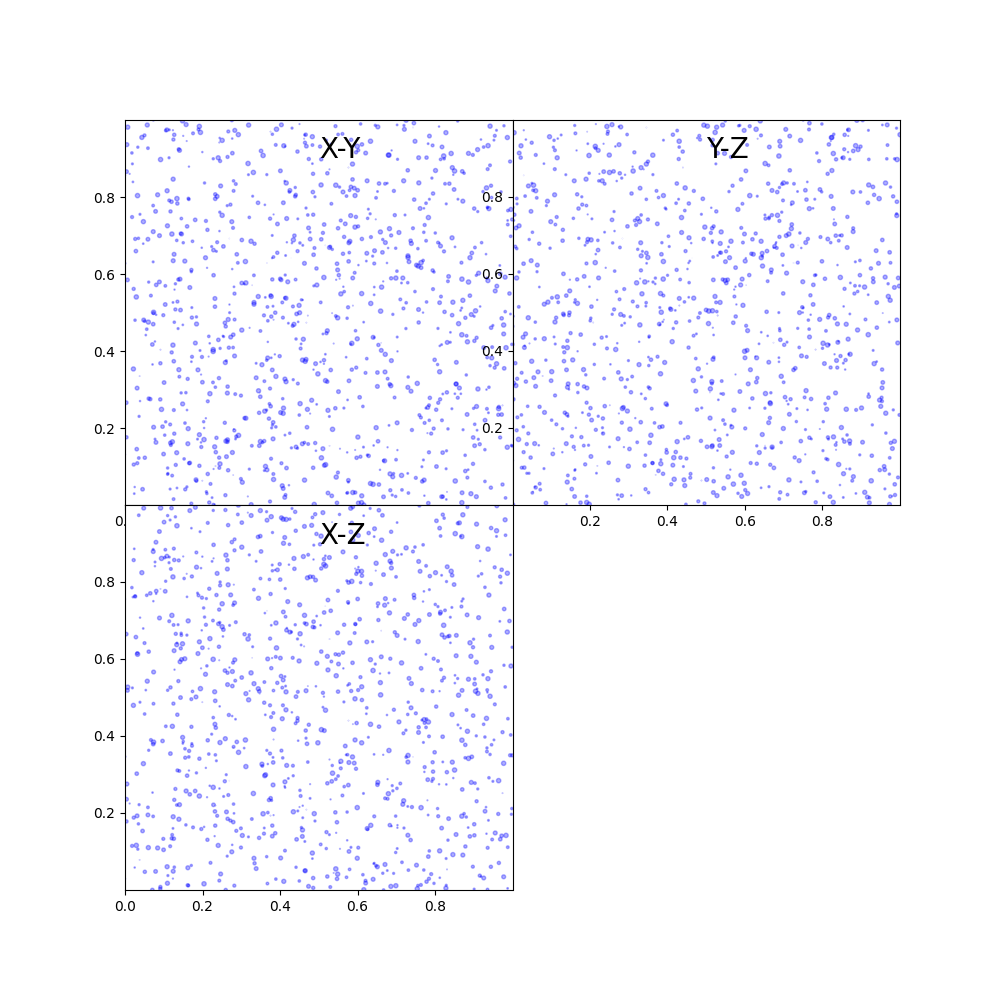
\includegraphics[width=0.4\textwidth, valign=c, clip=true trim=40.cm 2.cm 20.cm 2.cm]{figs/nbody-scatter-plot.t-i.png}
	% 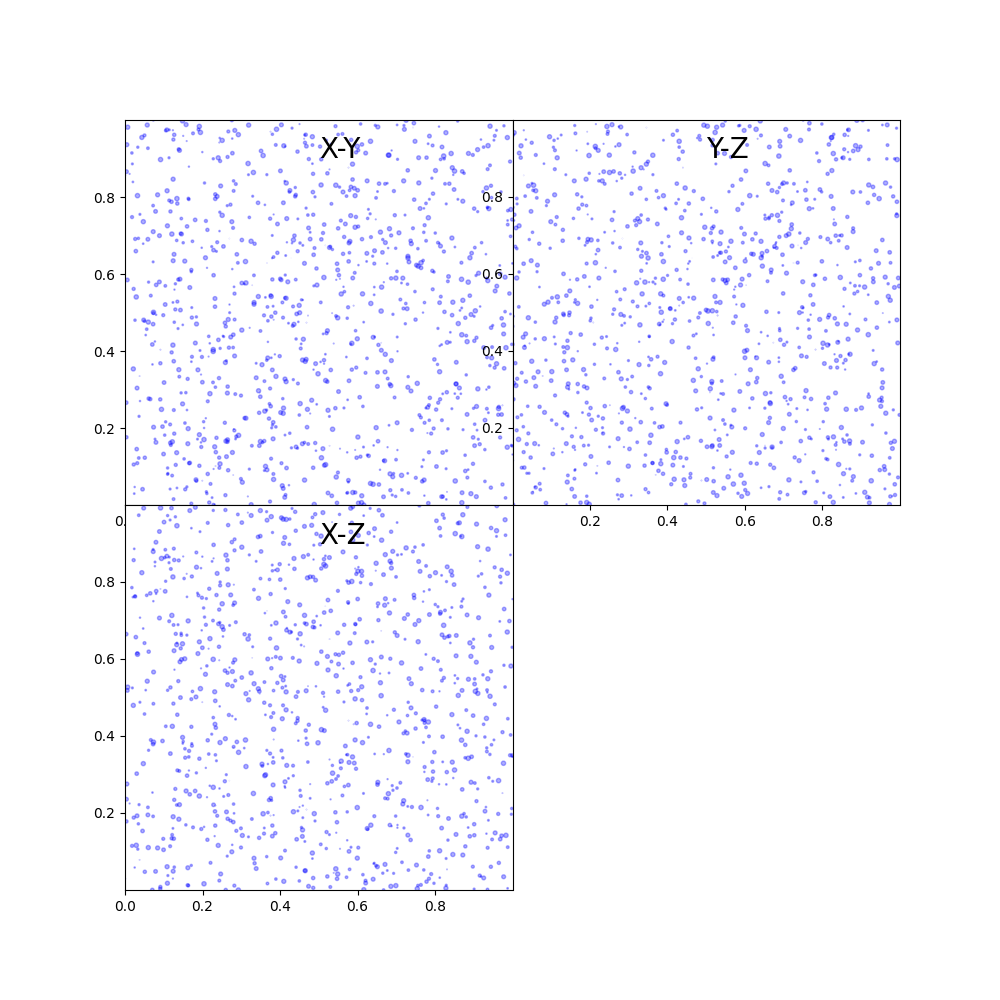
\includegraphics[width=0.4\textwidth, valign=c, clip=true trim=2.cm 2.cm 2.cm 2.cm]{figs/nbody-scatter-plot.t-f.png}
	% 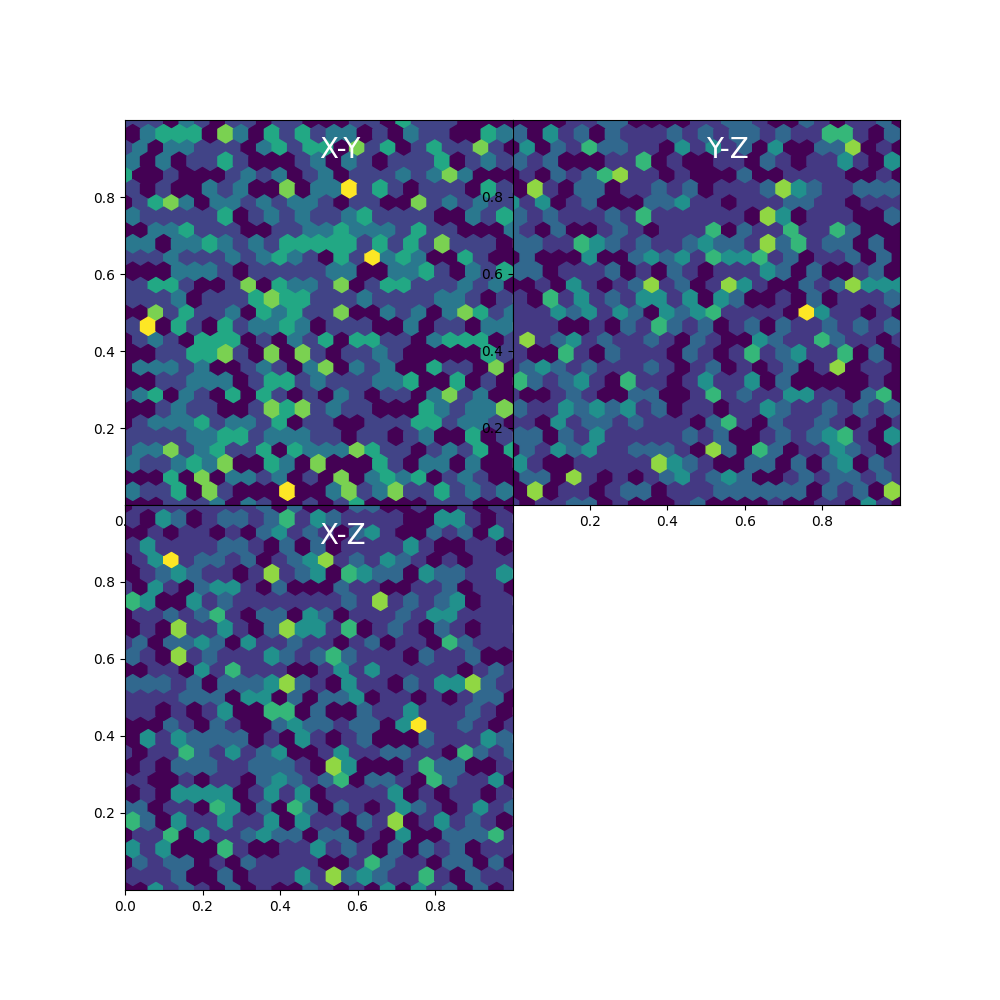
\includegraphics[width=0.4\textwidth, valign=c, clip=true trim=2.cm 2.cm 2.cm 2.cm]{figs/nbody-density-plot.t-i.png}
	% 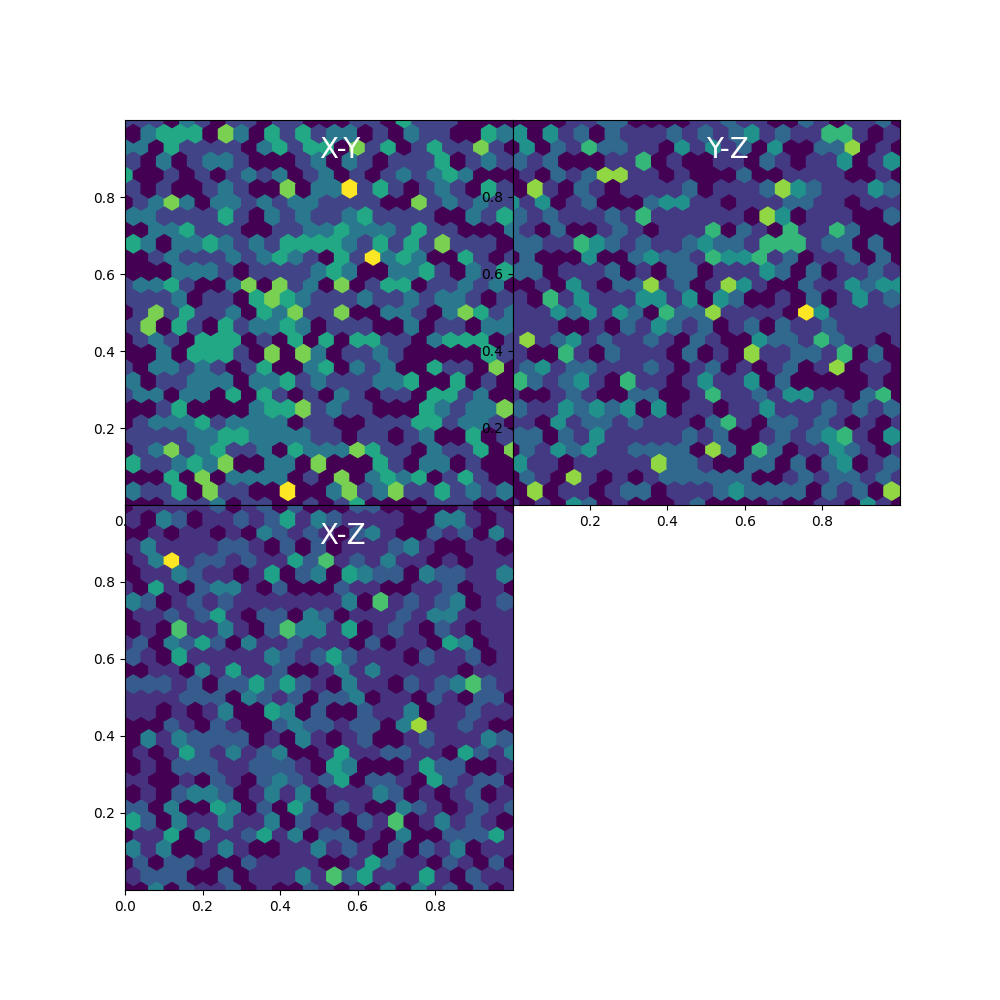
\includegraphics[width=0.4\textwidth, valign=c, clip=true trim=2.cm 2.cm 2.cm 2.cm]{figs/nbody-density-plot.t-f.png}
\end{minipage}
\end{center}

\subsection{Compiling on Pawsey systems}
The serial fortran codes will compile with all compilers on \texttt{setonix} so long as the appropriate compiler for the given programming environment is chosen. The make commands to use are 
\begin{itemize}
    \setlength{\itemindent}{70pt}
    \item[\texttt{PrgEnv-cray}:\quad]{\texttt{make COMPILERTYPE=CRAY}}
    \item[\texttt{PrgEnv-gnu}:\quad]{\texttt{make COMPILERTYPE=CRAY-GNU}}
\end{itemize}
On other machines that do not make use of the Cray compiler wrappers, it is just a matter of specifying the appropriate compiler such as \texttt{make COMPILERTYPE=GNU} for \texttt{gnu} compilers.
